\documentclass[../main.tex]{subfiles}

\begin{document}
\label{sec:fpc}

The paper~\cite{popov2019} introduces a protocol 
of low communicational complexity
which allows a set of nodes to come to a 
consensus on a value of a bit by means 
of (possibly randomized) voting
(see e.g.,~\cite{Becchetti2016,cooper2014,cooper2015, elsasser2016,fanti2019,mallmann2017}
and references therein for the vast available literature 
on this subject). The FPC relies on the idea that randomised voting, i.e., random queries, is in some situations sufficient for good performance, and due the small message complexity the protocol becomes scalable. Another advantage of this randomness is robustness in less reliable networks and in situations with inevitable churns (nodes join and leave), e.g.,~we refer to \cite{wang2017probabilistic} for an application of this idea in distributed machine learning. 

We mention also the classical work on (probabilistic)
Byzantine consensus protocols,
see e.g.,~\cite{AguTou12, Ben83, Bra87, CasLis02, 
FelMic89, FriMosRay04, Rab83}, where,
typically, the communicational complexity is much larger.

In order to  analyze  the security of FPC, we must define our assumptions about the behaviors of the participants in the system. An \emph{honest} participant is one that we assume to follow the system’s protocol rules as specified, hence representing a participant exhibiting no adversarial behavior.~A \emph{Byzantine} (a.k.a.,~\emph{active} or \emph{malicious}) participant is one we make no assumptions about; such a participant can behave in arbitrary fashion, without any restriction. Since this is the strongest adversarial model we will focus primarily on Byzantine attacks. We further assume that the Byzantine attacker is \emph{omniscient}, i.e.,  it is aware of the current opinion of every other node and observes all communications\footnote{This is one reason why we do not consider \emph{honest-but-curious}  (a.k.a.,~\emph{passive} or \emph{semi-honest}) adversaries separately.}
and that the adversary is \emph{rushing}, i.e., it may delay sending its own messages in any given round until after the honest parties send their messages in that round. %Finally, we assume the adversary to be \emph{computationally unbounded}. 
We refer to \cite{Ford2019} for more details on threat modeling and different kind of attackers. 

We have to make assumptions on the communication model of the FPC. We assume the communication between two nodes to satisfy \emph{authentication}, i.e., senders and receivers are who they claim to be, and \emph{data integrity}, i.e., data is not changed from source to destination. As we consider omniscient adversaries we do not assume \emph{confidentiality}. 
For the communication of the opinions between nodes we assume a  \emph{probabilistic synchronous model}, in which for every $\varepsilon>0$ and $\gamma>0.5$, a majority proportion $\gamma$ of the messages  is delivered within a bounded (and known) time, that depends on $\varepsilon$ and $\gamma$, with probability of at least $1-\epsilon$. We want to emphasize that, due to its random nature, FPC still shows good performances in situations where not all queries are answered in due time.






The aim is to build systems that could withstand the most  participants being Byzantine. In practice we have  to make threshold security assumptions, such as that over half or over two-thirds of the participants  are honest. 
The distinguishing feature of the mechanism described in~\cite{popov2019}
is that a larger number of
adversarial (or Byzantine)
 nodes is allowed, which may be a (fixed)
proportion of the total number of nodes.
Those adversarial nodes 
intend to either delay the consensus,
or break it (i.e., make at least a couple of honest nodes
come to different conclusions).
 It is shown that,
nevertheless, the protocol works with high probability
 when its parameters
 are suitably chosen, and  
some explicit estimates on the probability 
that the protocol finalizes in the consensus state
in a given time are also provided (see Theorems~2.1
and~2.4 of \cite{popov2019}).

Differently from the classical work
in this area, 
it is not required that
the consensus should be achieved, with high probability, on the initial majority
value.
Rather, 
\begin{itemize}
 \item if, initially, no 
 \emph{significant majority}\footnote{Loosely speaking,
 a significant majority is something statistically 
 different from the $50/50$ situation; for example,
 the proportion of $1$-opinion is greater than~$\phi$
 for some fixed $\phi>1/2$.} 
 of nodes prefer~$1$,
 then the final consensus will be on the value~$0$ 
with high probability;
 \item if, initially, a 
 \emph{supermajority}\footnote{Again, this is 
 a loosely defined notion; 
 a supermajority is something already \emph{close}
 to consensus, e.g., more than 90\% of all nodes 
 have the same opinion.}
 of nodes prefer~$1$,
 then the final consensus will be~$1$ with high probability.
\end{itemize}
To explain why this is relevant in cryptocurrency 
applications, consider a situation when there 
are two contradicting transactions;
for example, one of them transfers all the balance of 
address~$A_1$ to address~$A_2$, while the other
transfers all the balance of 
address~$A_1$ to address~$A_3\neq A_2$.
In the case when neither of the two transactions
is strongly preferred by the nodes of the network,
by declaring both invalid we are on the safe side.
On the other hand, it would not be a good idea to \emph{always}
declare them invalid. Indeed, if we do this, 
then a malicious actor would be able to 
exploit it in the following
way: First, he places a legitimate transaction, e.g.,\
to buy some goods from a merchant. When he receives 
the goods, he publishes a double-spending transaction
as above in the hope that \emph{both} would be
canceled by the system, and so he would effectively
receive his money back (or at least take
the money away from the merchant). To avoid this kind
of development, it would be desirable if the first
transaction (payment to the merchant) which,
by that time, have probably gained some confidence 
 from the nodes, would stay confirmed,
and only the subsequent double-spend gets canceled.




A special feature of the protocol of~\cite{popov2019} is that it makes 
use of a sequence of random numbers which are either
provided by a trusted source~\cite{nist:2019} or generated
by the nodes themselves using some
decentralized random number generating protocol 
(provided that the proportion of the adversarial nodes is not too large) 
by leveraging on cryptographic primitives such as verifiable secret sharing, 
threshold signatures, cryptograhic sortition or verifiable delay functions,
see e.g.,~\cite{cascudo2017, popov2017, schindler2018, syta2017, gilad2017algorand, boneh2018}.
More specifically, a reasonable approach could be to use a variant of the \emph{drand} protocol\footnote{\url{https://github.com/dedis/drand}} (already used by other projects such as \emph{The League of Entropy}\footnote{\url{https://www.cloudflare.com/leagueofentropy/}}) as detailed in a post on \emph{iota.cafe}\footnote{\url{https://iota.cafe/t/distributed-random-number-generator/243}}.
%


It is important to observe that,
even if from time to time the adversary can get
(total or partial) control 
of the random number, this can only lead to delayed consensus,
but he cannot convince different honest nodes of different 
things, i.e., safety is not violated.
Also, it is not necessary that really \emph{all}
honest nodes agree on the same number; if most 
of them do, this is already enough for the 
protocol (that is, the specific task
of random number generation does not require
any sort of ``strong consensus''). Similarly a random number is also not required for every round, see Fig. 17 in \cite{FPCsim2019}.

\subsubsection{The base protocol}
We present here only some key elements of the proposed
protocol and refer the interested reader to~\cite{FPCsim2019} and \cite{popov2019} for more details. In order to define FPC we have to  introduce some notation.
We assume the network to have $n$ nodes indexed by $1,2,\ldots, n$.\footnote{This assumption is only made for sake of a better presentation; a node does not need to know every other node in the network. While the theoretical results in \cite{popov2019} are proven under this assumption, simulation studies \cite{FPCsim2019} indicate that it is sufficient if every node knows about half of the other nodes.}  Every node $i$ has an opinion or state. We note $s_{i}(t)$ for the opinion of the node $i$ at time $t$. Opinions take values in $\{0,1\}$.


At each (discrete) time step each node chooses $k$ random nodes $C_{i}$, queries their opinions and calculates 
\begin{equation*}
\eta_{i}(t+1)=\frac1{k_{i}(t)} \sum_{j\in C_{i}} s_{j}(t),
\end{equation*}
where $k_{i}(t)\leq k$ is the number of replies received by node $i$ at time $t$ and $s_j(t)=0$ if the reply from $j$ is not received in due time. 
Note that the neighbors $C_{i}$ of a node $i$ are chosen using sampling with replacement and hence repetitions are possible.


As in \cite{FPCsim2019} we consider a basic version of the FPC introduced in \cite{popov2019} in choosing some parameters by default. Specifically, we remove the cooling phase of FPC and the randomness of the initial threshold $\tau$. Let $U_{t}, t=1, 2,\ldots$ be i.i.d.~random variables with law $\mathrm{Unif}( [\beta, 1-\beta])$ for some parameter $\beta \in [0,1/2]$. The update rules for the opinion of a node $i$ is given by
\begin{equation*}
s_{i}(1)=\left\{ \begin{array}{ll}
1, \mbox{ if } \eta_{i}(1) \geq \tau, \\
0, \mbox{ otherwise,}
\end{array}\right. 
\end{equation*}
and for $t\geq 1$:
\begin{equation*}
s_{i}(t+1)=\left\{ \begin{array}{ll}
1, \mbox{ if } \eta_{i}(t+1) > U_{t}, \\
0, \mbox{ if } \eta_{i}(t+1) < U_{t}, \\
s_{i}(t), \mbox{ otherwise.}
\end{array}\right. 
\end{equation*}
Note that if $\beta=0.5$, FPC reduces to a standard majority consensus. The above sequence of random variables $U_t$ are the same for all nodes, see also the discussion in the previous section.

We introduce a local termination rule to reduce the communication complexity of the protocols. Every node keeps a counter variable \verb?cnt? that is incremented by $1$ if there is no change in its opinion and that is set to $0$ if there is a change of opinion. Once the counter reaches a certain threshold $\verb?l?$, i.e.,~$\verb?cnt?\geq \verb?l?$,  the node considers the current state as final. The node will therefore no longer send any queries but will still answer incoming queries. In absence of autonomous termination the algorithm is halted after $\verb?maxIt?$ iterations.  

\subsubsection{Byzantines adversaries}
We consider the ``worst-case'' scenario where adversarial nodes can exchange information freely between themselves and can agree on a common strategy. In fact, we assume that all Byzantine nodes are controlled by a single  adversary.  In~\cite{popov2019}, three different kinds of these Byzantine adversaries are described and analyzed in more detail:% We therefore subdivide the Byzantine adversaries into:
\begin{itemize}
\item \emph{Cautious} adversary: any adversarial node must maintain the same opinion in the same round, i.e., respond the same value to all the queries it receives in that round;
\item \emph{Semi-cautious} adversary: adversarial node will not give contradicting responses, however if it suits them they may not respond to a node;% Due to the lack of response to individual nodes the effects may be similar to a berserk attack although the impact would be less severe. 
\item \emph{Berserk} adversary: an adversarial node may respond different opinions to different queries in the same round.
\end{itemize}



Since the berserk attack strategy allows more degrees of freedom in the possible responses of the adversary, it is the most problematic one.

\subsubsection{Theoretical analysis}
We present some theoretical results on FPC.  In \cite{popov2019} it is proven that, when the protocol parameters are suitable chosen, the protocol finalizes in a consensus state in finite time with high probability. We state a consequence of Theorems 4.1 and  6.2  in \cite{popov2019}.  
\newtheorem{theorem}{Theorem}
\begin{theorem}
Let $q$ be the proportion of adversarial nodes. Then, for any choice of $\varepsilon>0$, and 
\begin{enumerate}
    \item for any cautious adversary with $q<\frac12$,
    \item for any semi-cautious adversary with $q<\frac{1}{1+\varphi}\approx 0.38$\footnote{Interestingly, the golden ratio $\varphi=\frac{1+\sqrt{5}}2$ appears here.}, or
    \item for any berserk adversary with $q<1/3$,
\end{enumerate}
    there exist, for sufficiently large $n$, parameters $k, \beta, \verb?l?$ and $\verb?maxIt?$  such that the protocol finalizes in a consensus state with probability of at least $1-\varepsilon$.
\end{theorem}
The above results come with bounds on the values of the different parameters. Moreover, since these bounds are not yet optimal, simulations studies were performed in \cite{FPCsim2019} on various  explicit cautious and berserk adversarial strategies.
For instance, two strategies are presented in the study, where the attack aims for an agreement failure in the protocol: the cautious inverse voting strategy (IVS) and the berserk maximal variance strategy (MVS). In the IVS, the adversary transmits at time $t+1$ the opinion of the minority of the honest nodes of step $t$. In the MVS, the adversary waits until all honest nodes received opinions from all other honest nodes. The adversary then tries to subdivide the honest nodes into two equally sized groups of different opinions while trying to maximize the variance of the $\eta$-values. 



\begin{center}
\begin{minipage}{\textwidth}
     \hspace{0.5cm}
     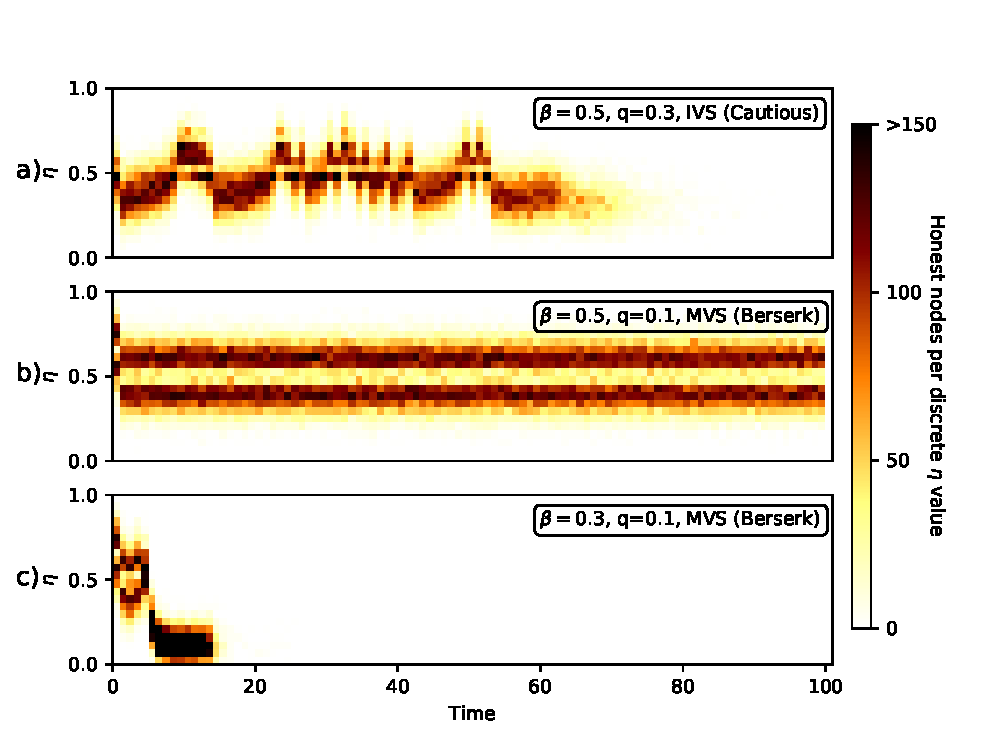
\includegraphics[scale=0.65]{images/epsHisto.eps}
     \captionof{figure}{Evolution of the received mean opinions $\eta$ of the number of undecided nodes. We consider a network of $n=1000$ nodes containing $qn$ malicious nodes and a quorum size of $k=21$. The  initial average opinion $p_0$ equals  the initial threshold $\tau=2/3.$}
     \label{fig:fpc_result1}
\end{minipage}\hfill
\end{center}

Fig.~\ref{fig:fpc_result1} compares the effects of the IVS and the MVS on the histogram evolution of the nodes’ received mean opinions $\eta$. In Fig.~\ref{fig:fpc_result1}a) and b) the randomization of the threshold is turned off. We show that the IVS is less efficient and the adversary struggles to keep the opinions split. On the other hand the berserk MVS strategy performs much better. Fig.~\ref{fig:fpc_result1}c) shows that when the random threshold is activated, the protocol performs well even against the berserk attack. 



Furthermore, optimisation studies show that an optimum range for the random threshold can be found, that maximizes the resilience to adversary nodes. For example, Fig.~\ref{fig:fpc_result2} shows the agreement rate\footnote{The agreement rate is the rate at which the protocol concludes with all nodes having the same opinion.} under a berserk MVS attack, against the random threshold window $\beta$ and the proportion of adversary nodes $q$. 

\begin{center}
\begin{minipage}{\textwidth}
     \centering
     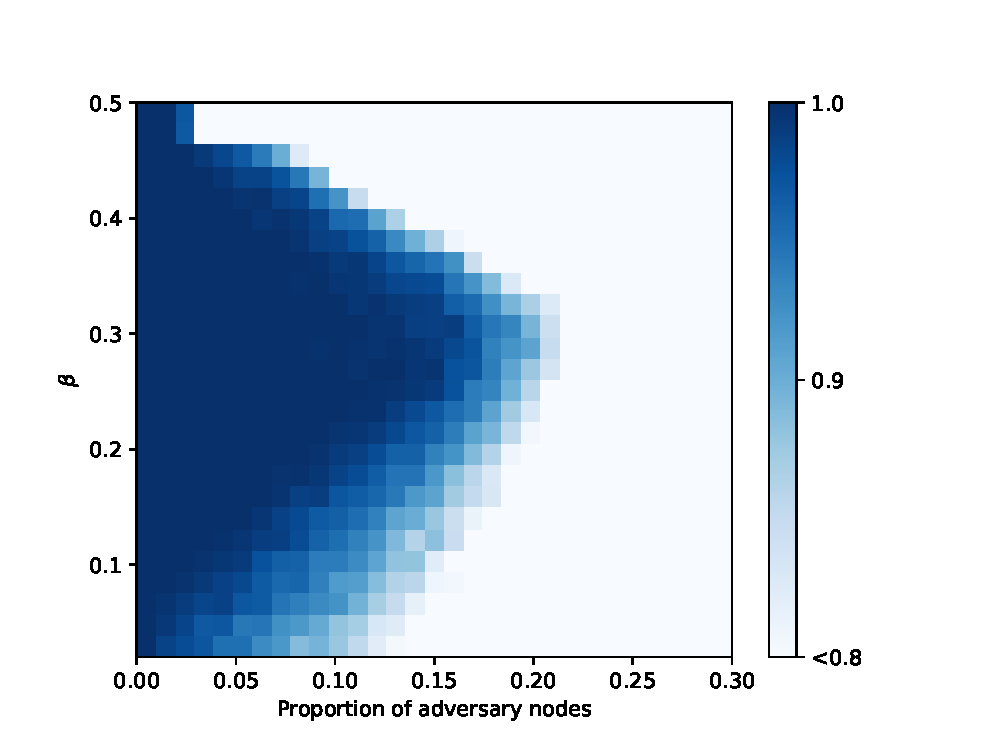
\includegraphics[scale=0.55]{images/2D__q_beta_agreement_2.eps}
     \captionof{figure}{Agreement rate against the parameter $\beta$ that decides the randomness of the threshold, and the proportion of MVS-adversarial nodes. We consider a network of $n=1000$ nodes containing $qn$ malicious nodes and a quorum size of $k=21$. The  initial average opinion $p_0$ equals  the initial threshold $\tau=2/3.$}
     \label{fig:fpc_result2}
\end{minipage}\hfill
\end{center}

Figs.~\ref{fig:fpc_result1} and \ref{fig:fpc_result2} show a worst case scenario in the following sense. The performances of the FPC are much better if the initial average opinion $p_0$ is not close to the initial threshold $\tau=2/3.$ It is also worth to note, that an increase of the quorum size $k$ leads to higher agreement rates and allows FPC to withstand higher proportion of adversarial nodes. 

\subsubsection{manaFPC}
FPC in its Vanilla version described in \cite{popov2019} is not robust against Sybil attacks since an adversary could deploy an excessively large number of nodes, thus inflating the value of $q$.
In Section~\ref{sec:sybil} Sybil protection is implemented by \emph{mana}.
We change  FPC such that a node is queried proportional to its mana and do allow to query a node multiple times. As multiple queries don't increase the message complexity (a node just counts the opinion multiple times without sending multiple queries), this allows creating a bigger quorum using the same communication overhead. In turn, a larger number of samples increases the safety of the protocol.  
In situations with heterogeneous mana distributions, nodes with high mana might be queried by a high number of  nodes. Such high-mana nodes are therefore incentivized to gossip their opinions or to publish them on the tangle as a data transaction.

To further decrease the message overhead when gossiping their opinions, nodes can apply monotonicity rules and compress their statements. For example, if a transaction is liked that contains two (liked) conflicts in its past, it would be sufficient to inform with the opinion on the former transaction. We dub these selected opinions, which effectively vote on the entire future or past of a transaction, state-votes. 


\end{document}